\section{Planning with Clearance Value Annotations}
\label{aha:planningwithannotations}
On a grid map, a clearance value is associated with each octile and is perhaps best explained as representing the length or width of a theoretical square bounding volume that begins at the tile being evaluated and is expanded until it intersects an obstacle. \\
Figure \ref{aha-fig:annotations} gives a quick overview of the idea. In \ref{aha-fig:annotations}(a) we present a simple map region and a traversable target tile with minimum clearance. (b) and (c) show the first two successful expansions of the bounding volume; the third (d), fails. In (e) we show the resultant annotations using a single-terrain capability on our two-terrain toy map example. Note that hard obstacles are black and their clearances omitted. Finally, In \ref{aha-fig:annotations}(f) we show a different set of annotations derived using two-terrain capability.

\begin{figure}[htbp]
       \caption{\emph{The annotation process (top). Annoating our example map using a single terrain capability (left)  and multi-terrain capability (right) } }
       \begin{center}
                       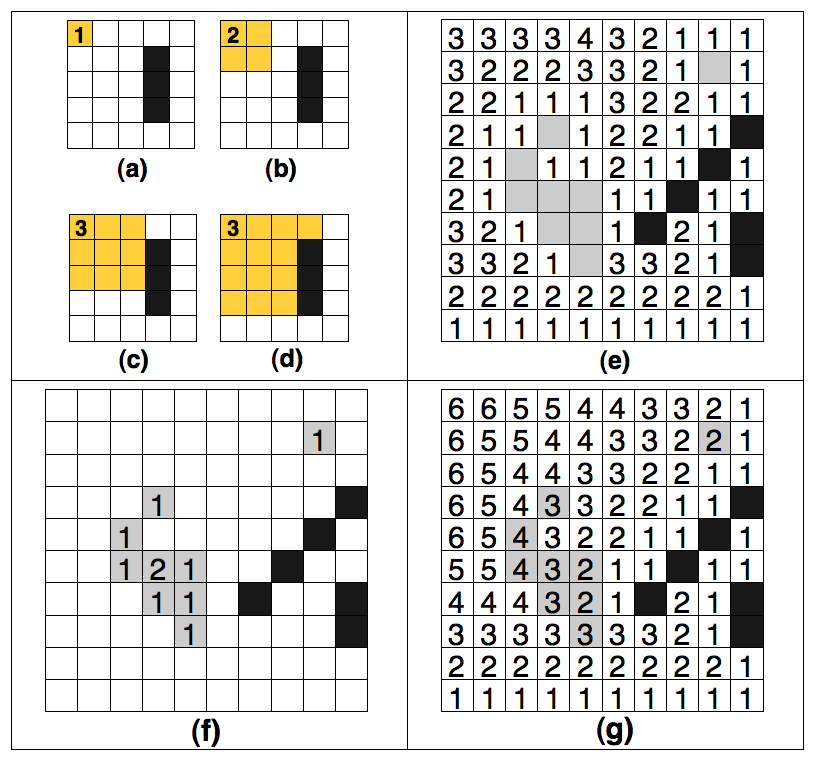
\includegraphics[scale=0.25]{diagrams/annotations.png}
       \end{center}
       \label{aha-fig:annotations}
\end{figure}

%\begin{figure}[htbp]
%        \caption{\emph{Determining maximal clearance} }
%        \begin{center}
%                        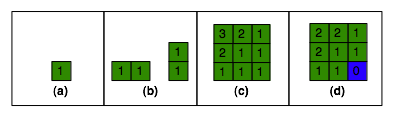
\includegraphics[scale=0.42]{diagrams/calculatingclearance.png}
%        \end{center}
%        \label{aha-fig:calculatingclearance}
%\end{figure}

In practice, we can more easily compute clearances recursively; we present such an implementation in algorithm \ref{aha-alg:calculateclearance}. The approach is straightforward:  
\begin{definition}
Each traversable tile begins with a minimum \emph{base clearance} of 1
\end{definition}

\begin{definition}
The clearance value of a traversable tile, for some capability $c$, is equal to its \emph{base clearance} + the minimum clearance value for $c$ among the set of immediate neighbours in the directions ${East, Southeast, South}$. We assume the map orientation is not isometric and up corresponds to the cardinal direction North. 
\end{definition}

\begin{definition}
All obstalces (hard or soft) have a clearance value of 0. 
\end{definition}

Once derived, we will use an additional few bytes of memory to annotate the corresponding node in our graph with this new information and repeat the entire procedure for each member in the set of all capabilities. Note that we do not need to store 0 values as the clearance for any capability which does not include a node's terrain is automatically 0 (ie. the node is a soft obstacle for any agent with  such capabilities). We omit precise implementation details of where to store clearances as these considerations will vary depending on the specific application and available resources. We opted to add attributes to our node data structures for simplicity; a better method would be to use compact tables.

\input algorithms/alg1_calculateclearance


\begin{lemma}
\label{aha-lemma:numannotations}
Let $r$ be the number of all terrain types in an environment, $V$ the set of all graph vertices and $V_{HO} \in V$ the set of hard obstacles. Then, the number of annotations required for a non-abstract graph is $|V|*2^r/2 - |V_{HO}|$
\end{lemma}

\begin{proof}
For a node to be traversable for some capability, the capability must include the node's terrain type (by definition). 
There are $2^r$ capabilities (by induction) but the maximum number of capabilities that include a node's terrain type is $2^r/2$ (by induction). There are $|V|$ nodes in total to represent the envrionment, and we avoid storing any clearance values for all nodes in $|V_{HO}|$. 
\qed
\end{proof}

The key advantage of annotating a map in this fashion is that we are able to plan for both large and small agents using a fixed size grid. 
We can determine valid pathfinding areas for any agent by simply comparing the size and capabilities of our agent with the corresponding terrain and capability clearance values in the search graph. 
In the case of large agents, we need know only that the top-left tile that will be occupied by the the agent is valid; the clearance value annotation guarantees that the rest of the area is obstacle free. This is an important property leading to reducibility and simplification of search problems. We give the following theorem and proof by contradiction:

\begin{theorem}
\label{aha-theorem:reducibility}
Given a suitably annotated grid map, any instance of of a large-agent search problem can be reduced into a small-agent search problem.
\end{theorem}

To prove theorem \ref{aha-theorem:reducibility}, we need to prove that it is always the case that the area represented by the clearance value of some node is obstacle free. 
\begin{proof}
It is not the case than an agent of some size and capability can successfully traverse an area represented by a node annotated with a clearance value at least equal to the agent's size. From this, it follows that one of the tiles in the area occupied by the agent is an obstacle for the agent (by definition). If one of the tiles occupied by the agent is an obstacle, it will have a clearance value of zero (by definition). Since the process for deriving clearance depends on recursively taking the minimum value among a set of neighbours, the clearance metric is measuring the distance to the nearest obstacle (intuitively, by definition). Thus, it cannot be the case that a node can have a larger clearance value than the minimum obstacle distance. This in turn means the agent cannot be occupying any tile which is an obstacle. \qed
\end{proof}
